\documentclass{article}

\usepackage[utf8]{inputenc}
\usepackage{setspace}
\usepackage[
	a4paper,
	total={17cm,25cm},
	top=3cm, left=2cm,
	includefoot
	]{geometry}
\usepackage[
	english,
	czech
	]{babel}
\usepackage[autostyle]{csquotes}
\usepackage{caption}
\usepackage{graphicx}
\graphicspath{{./assets/}}

\title{Správa Office 365}
\author{Petr Maronek}
\date{5.11.2022}

% 	Vysvětlivky
%	\section* hvězdička znamená, že má LaTeX odebrat číslování

\begin{document}
	\begin{spacing}{1.15}
		\rmfamily
		\maketitle
		\begin{center}
			\textbf{Vysoká škola finanční a správní}\linebreak
			Projektování Informačních Systémů 1\linebreak
			Zimní semestr 2022\linebreak
			Vedoucí práce: \textbf{Ing. Václav Řezníček, Ph.D.}
		\end{center}
		\pagebreak
			
		\section*{Abstrakt}
		Návrh zlepšení procesu pro správu Microsoft Office 365, která již vykazuje známky stárnutí technologie. to může vézt až ke výrazné ztrátě firemních finančních prostředků.
		 
		\section*{Klíčová slova}
		Office365, Microsoft, proces, automatizace, korporace, cloud
		\pagebreak
		    
		\section*{Úvod}
		Hra je postavená na \textbf{blockchain} technologii. Níže je zobrazena myšlenková mapa, která zobrazuje prvky hry.\linebreak
		
		\label{Myšlenková mapa}
		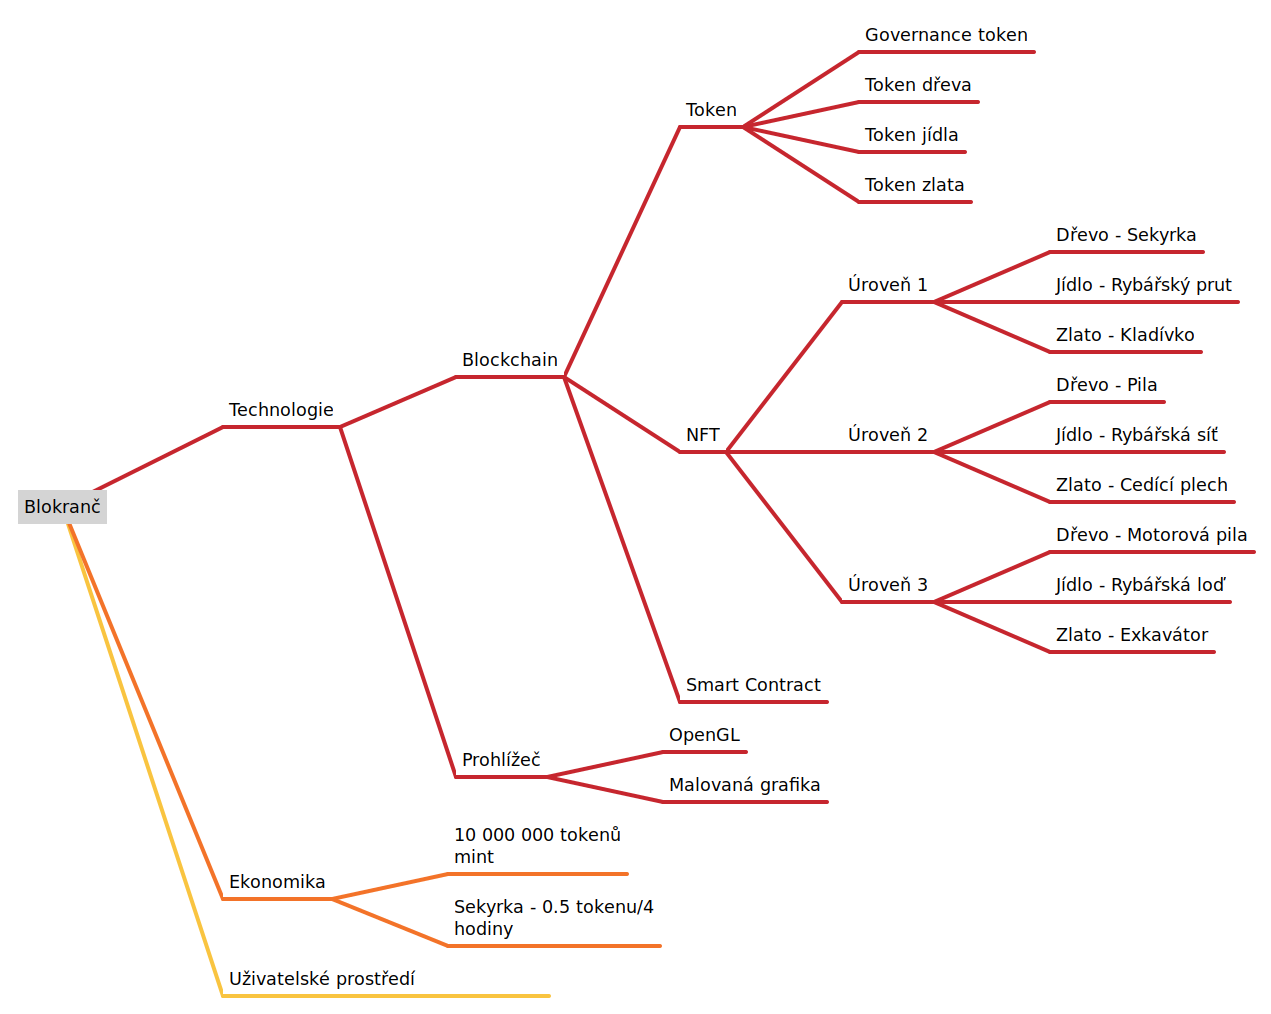
\includegraphics[scale=0.3]{221104-NPH-Blokranč.png}
		\captionof{figure}{Myšlenková mapa}
		
		A pokračujeme v textu dál.
	
	\end{spacing}
\end{document}

